% ~~~ [ Control Flow Analysis ] ~~~~~~~~~~~~~~~~~~~~~~~~~~~~~~~~~~~~~~~~~~~~~~~~

\subsubsection{Control Flow Analysis}
\label{sec:design_control_flow_analysis}

The control flow analysis component produces structured CFGs (in JSON format) from unstructured CFGs (in the DOT file format), by identifying high-level control flow primitives within the graph. The control flow structure is recorded by relating each node of the CFG to a specific node within the graph representation of a high-level control flow primitives, as illustrated in figure \ref{fig:representation_and_identification_of_primitive}.

\begin{figure}[htbp]
	\centering
	\begin{subfigure}[ht]{0.10\textwidth}
		\lstinputlisting[language=go, style=go, breaklines=false, numbers=none]{poster/inc/if.c}
		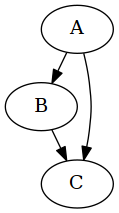
\includegraphics[width=\textwidth]{poster/inc/if.png}
	\end{subfigure}
	\enskip
	\begin{subfigure}[ht]{0.18\textwidth}
		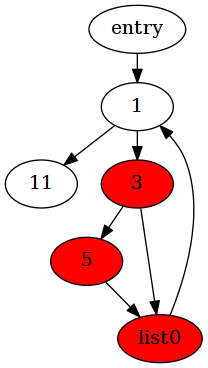
\includegraphics[width=\textwidth]{poster/inc/foo.png}
	\end{subfigure}
	\caption{The left side contains the pseudo-code (top left) and graph representation (bottom left) of an if-statement; if \texttt{A} is true then do \texttt{B} followed by \texttt{C}, otherwise do \texttt{C}. The right side highlights (in red) an identified isomorphism of the if-statement's graph representation in the CFG of a simple function.}
	\label{fig:representation_and_identification_of_primitive}
\end{figure}

% The \texttt{restructure} tool searches for subgraph isomorphisms of control flow primitives in a given CFG. Once located the nodes identified subgraph are merged into a single node which is labeled with the high-level control flow primitive. Successive iterations continue to simplify the CFG until only one node is left, at which point the high-level control flow primitive has been recovered. Should the \texttt{restructure} tool fail to reduce the graph into a single node, the graph is considered irreducible with regards to the supported high-level control flow primitives.

%TODO: Add: A data-driven design separates data from source code to facilitate the extensibility of components.

% TODO: Refer back to "each with access to the least amount of information required to successfully accomplish its task". Working on CFG, oblivious to the presence of LLVM IR or instructions for that matter.

% * Data-driven Design (potential and limitations)
% TODO: Mention: CFG invariants (e.g. single-entry, single-exit)

% TODO: Add: Limitations

% TODO: Add limitations related to the design choices. Which limitations are easily solvable given more time and which are fundamentally part of the design.
%    - No support for n-way conditionals (e.g.switch-statements). Potential solution: Domain Specific Language; e.g. switch could be written as:
%
%    digraph switch {
%       A -> B [label="expr='n > 2'; label='case %d'"]
%       A -> C
%       B -> C
%    }
%    - No support for inf-loops (because of the CFG invariant). Potential solution: relax invariant to support control flow primitive descriptors which only specify an entry node? These control flow primitives would have to be marked as no-exit.

%    - Unstructured CFG -> Structured CFG ([restructure](http://decomp.org/x/graphs/cmd/restructure).)

%The control flow analysis component structures low-level code by identifying high-level control flow primitives in the CFGs generated from LLVM IR (see section \ref{sec:design_control_flow_graph_generation}). As demonstrated in figure \ref{fig:representation_and_identification_of_primitive}, high-level control flow primitives may be represented using graphs. The problem of structuring low-level code may therefore be reformulated as the problem of locating subgraphs (e.g. the graph representations of control flow primitives) in graphs (e.g. the CFGs of low-level code) without considering node names. This problem is generally referred to as \textit{subgraph isomorphism search} and has been well studied \cite{subgraph_isomorphism_algorithms}.
